
\subsection{Reconstructing the Scalar Fields} % (fold)
\label{sec:reconstruction}
%
\Todo[inline]{Move the part about reconstruction and performance to the back}
%
If desired, the scalar fields on the original grid can be reconstructed from the
sparse representation by interpolation. We sample the fitted models in regular
intervals between the respective $x_l$ and $x_r$ of each line and variable. We
then apply standard interpolation methods to this set of points to reconstruct
the data on the original grid.

% Remember that when extracting the profiles, we deliberately ignored all
% data farther away from the flame surface than half the length of the sampled
% line. When reconstructing the data, we therefore only consider the region inside
% the convex hull of the point cloud resulting from sampling the fitted model
% functions. The remaining volume is assumed to contain only constant values.
%
% The interpolation scheme employed here has to be able to handle scattered data,
% must be efficient, and has to produce results as close as possible to the
% original data. There are generally three approaches for interpolating scattered
% data: Using a global method and generating new values from a combination of all
% data points, using only the local $k$ nearest data points to do the same, or
% generating a mesh with the data points as vertices and interpolating values
% inside the resulting cells using some mesh interpolation scheme. Global methods
% are not suitable here, as they are very inefficient. For each value that is
% interpolated, an expression involving all data points has to be evaluated. 

We compared two local interpolation methods for scattered data. The first method
is a \ac{kANN}~\cite{Arya1998} interpolation
scheme that weighs the values of the $k$ approximate nearest neighbors using
Shepard's inverse distance weights. 
%
% For large $k$ the result converges to the
% global Shepard interpolation but computation time increases. For small $k$ the
% computation is faster but the result has more discontinuities where the sets of
% nearest neighbors change.
%
% \begin{equation}
% \label{eqn:shepardweights}
% 	f(\vx) = \sum_{j=1}^k \frac{w_{i_j}(\vx)f_{i_j}}{\sum_{l=1}^k w_{i_l}(\vx)}, ~
% 	\text{with} ~ w_{i_j}(\vx) = \frac{1}{||\vx-\vx_{i_j}||^p}
% \end{equation}
% and $i_j, ~j=1,\dotsc, k$ are the indices of the $k$ approximate nearest
% neighbors of $\vx$.
% Since the $k$ approximate nearest neighbors can be found efficiently using a kd-
% tree and the Shepard weights are easily computable, this method is very fast.
%
The second interpolation method first generates a tetrahedral mesh from the data
points using a Delaunay triangulation. The values inside the mesh cells are then
linearly interpolated. This always produces a continuous solution if there are
no degenerate mesh cells.

Interpolation methods providing higher smoothness exist. However, these are more
computationally expensive and it is not guaranteed that they produce results
closer to the original data than the simpler methods.

\subsection{Quality and Performance Evaluation} % (fold)
\label{ssec:evaluation_compression}

% Evaluation of compression scheme to assess compression errors
% Used three different data sets
% describe data sets
%
We evaluated the accuracy of the sparse representation on single time steps of
three data sets. Each time-step of data sets \textsc{Syngas~I} and
\textsc{Syngas~II} has $\text{200}^3$ voxels and 13 variables each.
\textsc{Syngas~III} has $\text{100}^3$ voxels and 3 Variables. All data sets
are from \ac{DNS} computations of turbulent premixed spherical syngas flames.
\textsc{Syngas~I} contains a flame with strong wrinkles. \textsc{Syngas~II} has
a flame with smaller wrinkles. \textsc{Syngas~III} contains a flame that has
been torn into smaller parts by turbulence.
%
% Data sets \textsc{Syngas~I} and \textsc{Syngas~II} are from DNS
% computations of turbulent premixed spherical syngas flames. Each time-step has
% $200^3$ voxels and $13$ variables each. Data set \textsc{Hydrogen} is from a
% turbulent premixed spherical hydrogen flame and has a resolution of $400^3$
% voxels and $11$ variables. This is a size our application partner routinely uses
% for simulations. \textsc{Syngas~I} contains a flame with strong wrinkles.
% \textsc{Syngas~II} has a flame with smaller wrinkles. \textsc{Hydrogen} is much
% bigger but with a less wrinkled surface.
%
%, which yields a very similar surface, is used instead.
%
% 1. Errors made by fitting the models to the profile lines (\ac{RMS} error)
% Normalized by data value range to make comparable
% Shows raw error of models
% Results show low percentual errors for all variables

First, we investigate the error from approximating the original data by our
models. We computed the average \ac{RMS} error between the
original data of the profiles and the fitted models. The data values in the
range $x_{li}$ and $x_{ri}$ on each profile line are considered.
%
%(Figure~\ref{fig:models}), because values outside of this interval were not considered when fitting the models.
%
We used normalized \ac{RMS} errors $E^V_{\text{fit}}$ in order to make the
variables $V$ comparable:
%
%To make the values comparable, the resulting average
%\ac{RMS} error for each variable was normalized by the range of its values.
%The fitting error for a variable $V$ is then:
%
\begin{equation}
	E^V_{\text{fit}} 
		= 	\frac{(\max(V)-\min(V))^{-1}}{\sum_{i=1}^n x_{ri}-x_{li}} 
			\sum_{i=1}^n~
			\sum_{\{j | x_{li} \leq x_{ji} \leq x_{ri}\}}
						\frac{|P_{ij}^V-u_{ij}^V|}
							{x_{ri}-x_{li}} 
	\text{ .}
\end{equation}
\Todo{Check if equation is correct}
%
Here, $u_{ij}^V$ is the value of the fitted model corresponding to the original
profile value $P_{ij}^V$, while $\{j | x_{li} \leq x_{ji} \leq x_{ri}\}$ are the
indices of all points on the profile between $x_{li}$ and $x_{ri}$. We computed
this error for all possible profile lines in all data sets.
% 
% For smoothing the profiles before finding the feature points, we used a
% Gaussian kernel with $\sigma = 1 \text{ voxel}$.
%
As \cref{fig:fitting_rms_error} shows, the errors are quite low, ranging
from 0.1\% to 6.3\% of the respective variable's range.

For investigating the overall error after reconstruction, We computed the
reduction ratio $c$ for different $q$ and compared it to the
deviation from the original data after reconstruction. The reduction ratio is
defined as the storage space needed for the original data divided by the space
needed by the sparse representation.
%
% The most important
% measure for the quality of a lossy compression scheme is the relation of the
% reduction ratio to the compression error. In our approach, the compression
% ratio is determined by the number of profile lines seeded on the flame surface,
% and by the number and type of variables contained in the data set. The locations
% and directions of the profile lines $\vp_i$ and $\vr_i$ only have to
% be stored once for all variables. Thus, with more variables in the data set, the
% space needed for this information becomes less significant. Also, the more
% reactants and products are contained in the data set, compared to the number of
% intermediate species, the better the reduction ratio, since the sigmoidal
% model used for representing those species needs seven parameters, while the
% Gaussian model needs eight. 
% Most significant for the reduction ratio, however, is the number of seeded
% profile lines. This is steered by the value of $q$, but mainly
% depends on the data itself. Higher data resolution means that more lines are
% seeded. More importantly, the size and structure of the flame itself is
% responsible for the reduction ratio. A small flame naturally results in fewer
% profile lines seeded on its surface. If the flame is very smooth and does not
% exhibit a lot of wrinkles, fewer lines are seeded also, due to the low surface
% curvature. Big, strongly wrinkled flames will need much more profile lines to be
% represented accurately, resulting in a lower reduction ratio.
% \todo{explain this earlier. Especially emphasize data dependence of
% seeding and therefore reduction ratio.}
%
% \begin{equation}
% 	c 
% 		= \frac{B_\text{original}}{B_\text{sparse}} 
% \end{equation}
%
% Where $B_\text{original}$ and $B_\text{sparse}$ are the storage space needed to
% store the original and transformed data. 
%
% The sparse representation consists of the vertices and faces of the flame
% surface mesh, the indices of the vertices selected for seeding profiles, the
% directions $\vr_i$ of the profile lines, and the model parameters for each
% simulation variable and profile.
%
%For measuring the reconstruction error, we computed the mean square errors for
%ach variable in the data set after compressing and decompressing them.
%
%The error was normalized by the range of values of the variable, to make the errors
%for different variables comparable.
%
We used a normalized root mean square error metric to compute the reconstruction
quality:
%
\begin{equation}
	E^V_\text{reconst}
		= 	\frac{1}{|H|}
			\int\limits_{\vx \in H}
				\left|
					\frac{R(\vx) - V(\vx)}{\max(V)-\min(V)}
				\right| ~d\vx
			 \text{ ,}
\end{equation}
%
where $V$ is the original data of the variable, $R$ is the reconstructed data,
$H$ is the convex hull of all points used to reconstruct the data, and $|H|$ is
the volume of H. The range of values of variable $V$ is described by
$\max(V)-\min(V)$.

%
\begin{figure}[t]
	\centering
    \setlength\figureheight{0.2\textheight}
    \setlength\figurewidth{0.87\textwidth}
	%
%
% This file was created by matlab2tikz v0.4.0.
% Copyright (c) 2008--2013, Nico Schlömer <nico.schloemer@gmail.com>
% All rights reserved.
% 
% The latest updates can be retrieved from
%   http://www.mathworks.com/matlabcentral/fileexchange/22022-matlab2tikz
% where you can also make suggestions and rate matlab2tikz.
% 
\begin{tikzpicture}

\begin{axis}[%
small,
width=\figurewidth,
height=\figureheight,
area legend,
legend style={at={(0.98, 1.15)}, anchor=north east, legend columns=1, font=\small},
scale only axis,
axis y line = left,
axis x line* = bottom,
xmin=0.5,
xmax=13.5,
ylabel={$E^V_{\text{fit}}$},
every axis y label/.style={at={(current axis.above origin)},anchor=south east},
scaled y ticks = false,
yticklabel style = {/pgf/number format/precision=3, /pgf/number format/fixed},
ybar,
ymin=0,
ymax=0.085,
xtick={1,2,3,4,5,6,7,8,9,10,11,12,13},
xticklabels={OH,\ce{O2},O,\ce{HO2},HCO,\ce{H2O2},\ce{H2O},\ce{H2},H,\ce{CO2},CO,\ce{CH2O},T},
every tick/.style={color=black, thin},
x tick label style = {rotate=90},
]
\addplot[ybar,mycolor1,bar width=0.01\figurewidth,fill=mycolor1] 
coordinates
{(1, 0.0160108368686018)
(2, 0.0179611197947222)
(3, 0.0512353285580825)
(4, 0.0280660639669209)
(5, 0.0216726758682414)
(6, 0.0468526577521646)
(7, 0.0159317115163465)
(8, 0.0185940722130954)
(9, 0.0297375593011707)
(10, 0.019667950937967)
(11, 0.020793157135868)
(12, 0.000950809666194)
(13, 0.030076831585527)};
\addlegendentry{\textsc{Syngas I}}

\addplot[ybar,mycolor2,bar width=0.01\figurewidth,fill=mycolor2] 
coordinates
{(1, 0.0235)
(2, 0.0165)
(3, 0.0632)
(4, 0.0312)
(5, 0.0125)
(6, 0.0492)
(7, 0.0148)
(8, 0.0174)
(9, 0.0322)
(10, 0.0245)
(11, 0.0247)
(12, 0.0008)
(13, 0.0342)};
\addlegendentry{\textsc{Syngas II}}

\addplot[ybar,mycolor3,bar width=0.01\figurewidth,fill=mycolor3]
coordinates
{
(10, 0.0226)
(6, 0.0136)
(5, 0.0068)	
};
\addlegendentry{\textsc{Syngas III}}

% \addplot[ybar,mycolor3,bar width=0.01\figurewidth,fill=mycolor3] 
% coordinates
% {
% (13, 0.036749)
% (14, 0.032756)
% (15, 0.032433)
% (9, 0.050241)
% (8, 0.019321)
% (7, 0.016394)
% (6, 0.037397)
% (4, 0.040298)
% (3, 0.029779)
% (2, 0.015316)
% (1, 0.085694)
% };
% \addlegendentry{\textsc{Hydrogen}}

\end{axis}
\end{tikzpicture}%
	\caption{Mean \ac{RMS} fitting error for all variables. Note that not all data sets
	contain the same variables.}
	\label{fig:fitting_rms_error}
\end{figure}
%
% 2. Total errors (MSE, PSNR?) after reconstruction
% Compare different seeding densities and different interpolation schemes
% Naive downsampling of original data to same compression factor as reference
% Only consider data in convex hull of profiles
% Compared different parameters for k and p and selected best one in average for comparison
% naive downsampling better for low compression factors as to be expected
% Much lower error rates than naive downsampling for higher compression factors
% Linear better than knn except for few places
% Compression factors up to about 1:150 without terrible errors
%
\begin{figure}[p]
	\setlength\figureheight{0.26\textheight}
	\setlength\figurewidth{0.8\textwidth}
	% \input{figures/msevcr_stack_small.tikz}\\
	% \input{figures/msevcr_stack_data3_small.tikz}\\
	% \input{figures/msevcr_stack_data2.tikz}\\
	%
\pgfplotstableread{figures/mse1.csv}\dataI
\pgfplotstableread{figures/mse1_spiht.csv}\spihtI
\pgfplotstableread{figures/mse3.csv}\dataII
\pgfplotstableread{figures/mse3_spiht.csv}\spihtII
\pgfplotstableread{figures/mse2.csv}\dataIII
\pgfplotstableread{figures/syngas_100_spiht_errs.csv}\spihtIII
%
% \pgfplotstableread{
% 	q\\
% 	240\\
% 	58\\
% 	36\\
% 	23.3\\
% 	16\\
% 	11.5\\
% 	6.7\\
% 	4.7\\
% 	2\\
% 	1
% }\densities
%
% \pgfplotstableset{
% 	create on use/densities/.style={create col/copy column from table={\densities}{[index] 0}}
% }
%
\begin{tikzpicture}[
    line/.style={thick},
    O/.style={color=mycolor1},
    H/.style={color=mycolor2},
    CO2/.style={color=mycolor3},
    H2O2/.style={color=mycolor4},
    HCO/.style={color=mycolor5},
    linear/.style={line, solid},
    knn/.style={line, dashed},
    downsampling/.style={line, dotted},
    spiht/.style={line, dashdotted},
]

\pgfplotsset{
    small,
    legend style={
        font=\small,
        draw=none,
        legend pos = north west,
        legend cell align=left},
    title style={
        at={(0.5, 1)},
        anchor=north,
        inner sep=0pt,
        yshift=-3mm,
    },
    every tick/.style={color=black, thin},
	width=\figurewidth,
	height=\figureheight,
	scale only axis,
	xmode=log,
}

\begin{axis}[%
    name = syngas1,
    title={\colorbox{white}{\textsc{Syngas I}}},
    axis y line* = left,
    axis x line* = box,
    xmin=7.63070945311032,
    xmax=1037.11379310345,
    xmode=log,
    xminorticks=true,
    ymin=0,
    ymax=0.08,%0.35119633835835,
    ylabel={$e^V_\textnormal{reconst}$},
    every axis y label/.style={
        at={(ticklabel cs:0.5)},rotate=90,anchor=center},
    ytick={0,0.015,0.03},
    scaled y ticks = false,
    yticklabels={\textcolor{mycolor3}{$\text{CO}_2$},
    		 \textcolor{mycolor2}{H},
    		 \textcolor{mycolor1}{O}},
    ymajorgrids,
    extra description/.code={
    		\xdef\XMIN{\pgfkeysvalueof{/pgfplots/xmin}}
            \xdef\XMAX{\pgfkeysvalueof{/pgfplots/xmax}}
            \xdef\YMIN{\pgfkeysvalueof{/pgfplots/ymin}}
            \xdef\YMAX{\pgfkeysvalueof{/pgfplots/ymax}}
            },
]
    % dummy plots for legend
    \addplot[linear]
    coordinates{
    	(10, 0)
    	(11, 0)
    };
    \addlegendentry{linear interp.}
    \addplot[knn]
    coordinates{
    	(10, 0)
    	(11, 0)
    };
    \addlegendentry{k{\otherscshape{}ann} interp.}
    \addplot[downsampling]
    coordinates{
    	(10, 0)
    	(11, 0)
    };
    \addlegendentry{downsampling}
    \addplot[spiht]
    coordinates{
    	(10, 0)
    	(11, 0)
    };
    \addlegendentry{{\otherscshape 3d}-{\otherscshape spiht}}

    \addplot [CO2, linear, forget plot]
        table[x=compr, y expr=\thisrow{CO2_lin}+0.00]{\dataI};
    \addplot [CO2, knn, forget plot]
        table[x=compr, y expr=\thisrow{CO2_knn}+0.00]{\dataI};
    \addplot [CO2, downsampling, forget plot]
        table[x=compr, y expr=\thisrow{CO2_down}+0.00]{\dataI};
    \addplot [CO2, spiht, forget plot]
        table[x=compr, y expr=\thisrow{CO2}+0.00]{\spihtI};

    \addplot [H, linear, forget plot]
        table[x=compr, y expr=\thisrow{H_lin}+0.015]{\dataI};
    \addplot [H, knn, forget plot]
        table[x=compr, y expr=\thisrow{H_knn}+0.015]{\dataI};
    \addplot [H, downsampling, forget plot]
        table[x=compr, y expr=\thisrow{H_down}+0.015]{\dataI};
    \addplot [H, spiht, forget plot]
        table[x=compr, y expr=\thisrow{H}+0.015]{\spihtI};

    \addplot [O, linear, forget plot]
        table[x=compr, y expr=\thisrow{O_lin}+0.03]{\dataI};
    \addplot [O, knn, forget plot]
        table[x=compr, y expr=\thisrow{O_knn}+0.03]{\dataI};
    \addplot [O, downsampling, forget plot]
        table[x=compr, y expr=\thisrow{O_down}+0.03]{\dataI};
    \addplot [O, spiht, forget plot]
        table[x=compr, y expr=\thisrow{O}+0.03]{\spihtI};

\end{axis}

\begin{axis}[% --- CF
    xmin=\XMIN,
    xmax=\XMAX,
    ymin=\YMIN,
    ymax=\YMAX,
    ticklabel pos=right,
	axis y line* = right,
	axis x line = none,
	ytick={0,0.015,0.03, 0.045, 0.06, 0.075},
	scaled y ticks = false,
	yticklabel style = {/pgf/number format/precision=4,
						/pgf/number format/fixed}
]
\end{axis}

\begin{axis}[%
    name = syngas2,
    title={\colorbox{white}{\textsc{Syngas II}}},
    at = {(syngas1.below south west)},
    yshift=-0.2cm,
    height = 0.87\figureheight,
    anchor = north west,
    axis y line* = left,
    axis x line* = box,
    xmode=log,
    xmin=17.276,
    xmax=2120.3,
    xminorticks=true,
    every axis x label/.style={
        at={(ticklabel cs:0.5)},anchor=center},
    ymin=0,
    ymax=0.08,%0.35119633835835,
    ylabel={$e^V_\textnormal{reconst}$},
    every axis y label/.style={
        at={(ticklabel cs:0.5)},rotate=90,anchor=center},
    ytick={0,0.015,0.03},
    scaled y ticks = false,
    yticklabels={\textcolor{mycolor3}{$\text{CO}_2$},
        		 \textcolor{mycolor2}{H},
        		 \textcolor{mycolor1}{O}},
    ymajorgrids,
    extra description/.code={
    		\xdef\XMIN{\pgfkeysvalueof{/pgfplots/xmin}}
            \xdef\XMAX{\pgfkeysvalueof{/pgfplots/xmax}}
            \xdef\YMIN{\pgfkeysvalueof{/pgfplots/ymin}}
            \xdef\YMAX{\pgfkeysvalueof{/pgfplots/ymax}}
            },
    %legend style={legend pos = north west}
]

    \addplot [CO2, linear, forget plot]
        table[x=compr, y expr=\thisrow{CO2_lin}+0.00]{\dataII};
    \addplot [CO2, knn, forget plot]
        table[x=compr, y expr=\thisrow{CO2_knn}+0.00]{\dataII};
    \addplot [CO2, downsampling, forget plot]
        table[x=compr, y expr=\thisrow{CO2_down}+0.00]{\dataII};
    \addplot [CO2, spiht, forget plot]
        table[x=compr, y expr=\thisrow{CO2}+0.00]{\spihtII};

    \addplot [H, linear, forget plot]
        table[x=compr, y expr=\thisrow{H_lin}+0.015]{\dataII};
    \addplot [H, knn, forget plot]
        table[x=compr, y expr=\thisrow{H_knn}+0.015]{\dataII};
    \addplot [H, downsampling, forget plot]
        table[x=compr, y expr=\thisrow{H_down}+0.015]{\dataII};
    \addplot [H, spiht, forget plot]
        table[x=compr, y expr=\thisrow{H}+0.015]{\spihtII};

    \addplot [O, linear, forget plot]
        table[x=compr, y expr=\thisrow{O_lin}+0.03]{\dataII};
    \addplot [O, knn, forget plot]
        table[x=compr, y expr=\thisrow{O_knn}+0.03]{\dataII};
    \addplot [O, downsampling, forget plot]
        table[x=compr, y expr=\thisrow{O_down}+0.03]{\dataII};
    \addplot [O, spiht, forget plot]
        table[x=compr, y expr=\thisrow{O}+0.03]{\spihtII};

\end{axis}

\begin{axis}[% --- CF
	at = {(syngas1.below south west)},
    yshift=-0.2cm,
	height = 0.87\figureheight,
	anchor = north west,
    xmin=\XMIN,
    xmax=\XMAX,
    ymin=\YMIN,
    ymax=\YMAX,
    ticklabel pos=right,
	axis y line* = right,
	axis x line = none,
	ytick={0,0.015,0.03, 0.045, 0.06, 0.075},
	scaled y ticks = false,
	yticklabel style = {/pgf/number format/precision=4,
						/pgf/number format/fixed}
]
\end{axis}

\begin{axis}[%
    name = syngas3,
    title={\colorbox{white}{\textsc{Syngas III}}},
    at = {(syngas2.below south west)},
    yshift=-0.2cm,
    height = 0.87\figureheight,
    anchor = north west,
    axis y line* = left,
    axis x line* = box,
    xmin=55.6919459459459,
    xmax=3815.92962962963,
    xmode=log,
    xminorticks=true,
    xlabel={$c$},
    every axis x label/.style={
        at={(ticklabel cs:0.5)},anchor=center},
    ymin=0,
    ymax=0.08,
    ylabel={$e^V_\textnormal{reconst}$},
    every axis y label/.style={
        at={(ticklabel cs:0.5)},rotate=90,anchor=center},
    ytick={0,0.015,0.03},
    scaled y ticks = false,
    yticklabels={
    		 \textcolor{mycolor5}{HCO},
    		 \textcolor{mycolor4}{$\text{H}_{2}\text{O}_2$},
    		 \textcolor{mycolor3}{$\text{CO}_2$},},
    ymajorgrids,
    extra description/.code={
    		\xdef\XMIN{\pgfkeysvalueof{/pgfplots/xmin}}
            \xdef\XMAX{\pgfkeysvalueof{/pgfplots/xmax}}
            \xdef\YMIN{\pgfkeysvalueof{/pgfplots/ymin}}
            \xdef\YMAX{\pgfkeysvalueof{/pgfplots/ymax}}
            },
    %legend style={legend pos = north west}
]
    \addplot [CO2, linear, forget plot]
        table[x=compr, y expr=\thisrow{CO2_lin}-0.01]{\dataIII};
    \addplot [CO2, knn, forget plot]
        table[x=compr, y expr=\thisrow{CO2_knn}-0.01]{\dataIII};
    \addplot [CO2, downsampling, forget plot]
        table[x=compr, y expr=\thisrow{CO2_down}-0.01]{\dataIII};
    \addplot [CO2, spiht, forget plot]
        table[x=r, y expr=\thisrow{CO2}+0.03]{\spihtIII};

    \addplot [H2O2, linear, forget plot]
        table[x=compr, y expr=\thisrow{H2O2_lin}-0.005]{\dataIII};
    \addplot [H2O2, knn, forget plot]
        table[x=compr, y expr=\thisrow{H2O2_knn}-0.005]{\dataIII};
    \addplot [H2O2, downsampling, forget plot]
        table[x=compr, y expr=\thisrow{H2O2_down}-0.005]{\dataIII};
    \addplot [H2O2, spiht, forget plot]
        table[x=r, y expr=\thisrow{H2O2}+0.015]{\spihtIII};

    \addplot [HCO, linear, forget plot]
        table[x=compr, y=HCO_lin]{\dataIII};
    \addplot [HCO, knn, forget plot]
        table[x=compr, y=HCO_knn]{\dataIII};
    \addplot [HCO, downsampling, forget plot]
        table[x=compr, y=HCO_down]{\dataIII};
    \addplot [HCO, spiht, forget plot]
        table[x=r, y=HCO]{\spihtIII};
\end{axis}

\begin{axis}[% --- CF
	at = {(syngas2.below south west)},
    yshift=-0.2cm,
	anchor = north west,
	height = 0.87\figureheight,
    xmin=\XMIN,
    xmax=\XMAX,
    ymin=\YMIN,
    ymax=\YMAX,
    ticklabel pos=right,
	axis y line* = right,
	axis x line = none,
	ytick={0,0.015,0.03, 0.045, 0.06, 0.075},
	scaled y ticks = false,
	yticklabel style = {/pgf/number format/precision=4,
						/pgf/number format/fixed}
]
\end{axis}

\end{tikzpicture}%
	\caption{
	Error vs. reduction ratio for selected variables. The plots corresponding to
	each variable are shifted by a constant increment. The horizontal lines
	signify the zero-levels of the respective plots.}
	\label{fig:CRvMSE}
\end{figure}

% \begin{figure}[tb]
% 	\centering
% 	\setlength\figureheight{5cm} 
% 	\setlength\figurewidth{0.7\textwidth}
% 	\input{figures/msevcr_stack_data3_small.tikz}
% 	\caption{Error vs. reduction ratio (\textsc{Syngas II}). See Figure 
% 	\ref{fig:CRvMSE} for explanation.
% 	}
% 	\label{fig:CRvMSE3}
% \end{figure}

% \begin{figure}[tb]
% 	\centering
% 	\setlength\figureheight{5cm} 
% 	\setlength\figurewidth{0.7\textwidth}
% 	\input{figures/msevcr_stack_data2.tikz}
% 	\caption{Error vs. reduction ratio (\textsc{Syngas III}). See Figure 
% 	\ref{fig:CRvMSE} for explanation.
% 	}
% 	\label{fig:CRvMSE2}
% \end{figure}

\begin{figure}[tp]
	\centering
	\setlength\figurewidth\textwidth
	\begin{tikzpicture}[
        font=\small,
        thick,
        node distance=0mm,
        every node/.style={inner sep=0, outer sep=0},
        top label/.style={anchor=north west, xshift=0.3cm, yshift=-0.3cm},
        bottom label/.style={anchor=south west, xshift=0.3cm, yshift=0.3cm},
        title/.style={anchor=text, yshift=2.5mm}
    ]

    \node (h_orig) {
            
\includegraphics[width=\figurewidth,
                             trim=0 100 0 50,
                             clip]
                            {images/data3/H_orig_rdoryl.png}
    };
    \node[top label] at (h_orig.north west) {Original};
    \node[anchor=east, draw=black, inner sep=0.05mm] (cmap) at ($(h_orig.east) + (-1cm, 0)$) {
        \rotatebox{-90}{%
        
\includegraphics[width=2.5cm,height=0.25cm]{figures/rdoryl.png}%
        }%
    };
    \node[anchor=north west, xshift=1mm] at (cmap.north east) {max};
    \node[anchor=south west, xshift=1mm] at (cmap.south east) {min};

    \node[title] at (h_orig.north west) {
        \textsc{\normalsize Syngas II: $\text{H}$}
    };

    \node[anchor=north west, at={($(h_orig.south west) + (0, -2mm)$)}] (h_lin) {
            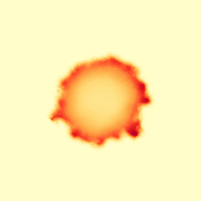
\includegraphics[width=0.33333333\figurewidth-1.3333333mm,
                             trim=30 100 30 30,
                             clip,
                             ]
                            {images/data3/H_lin_36_rdoryl.png}
    };
    \node[top label] at (h_lin.north west) {linear interpolation};

    \node[anchor=north, at={($(h_orig.south) + (0, -2mm)$)}] (h_knn) {
            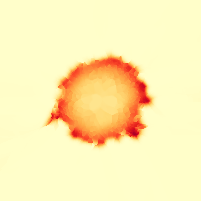
\includegraphics[width=0.33333333\figurewidth-1.3333333mm,
                             trim=30 100 30 30,
                             clip]
                            {images/data3/H_knn_36_rdoryl.png}
    };
    \node[top label] at (h_knn.north west) {k{\otherscshape{ann}} interpolation};

    \node[anchor=north east, at={($(h_orig.south east) + (0, -2mm)$)}] (h_down) {
            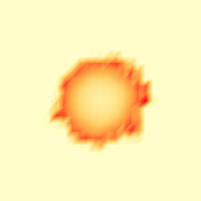
\includegraphics[width=0.33333333\figurewidth-1.3333333mm,
                             trim=30 100 30 30,
                             clip]
                            {images/data3/H_down_36_rdoryl.png}
    };
    \node[top label] at (h_down.north west) {downsampling};

    \node[anchor=north, at={(h_lin.south)}] (h_diff_lin) {
            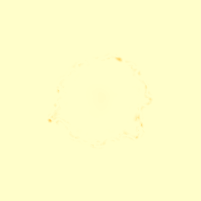
\includegraphics[width=0.33333333\figurewidth-1.3333333mm,
                             trim=30 30 30 100,
                             clip]
                            {images/data3/H_diff_lin_36_rdoryl.png}
    };
    \node[bottom label] at (h_diff_lin.south west) {
        $E^{\text{H}}_{\text{reconst}}$
    };
    \draw[dashed] (h_lin.south west) -- (h_lin.south east);

    \node[anchor=north, at={(h_knn.south)}] (h_diff_knn) {
            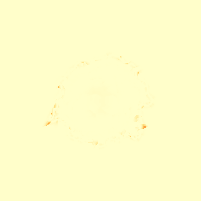
\includegraphics[width=0.33333333\figurewidth-1.3333333mm,
                             trim=30 30 30 100,
                             clip]
                            {images/data3/H_diff_knn_36_rdoryl.png}
    };
    \node[bottom label] at (h_diff_knn.south west) {
        $E^{\text{H}}_{\text{reconst}}$
    };
    \draw[dashed] (h_knn.south west) -- (h_knn.south east);

    \node[anchor=north, at={(h_down.south)}] (h_diff_down) {
            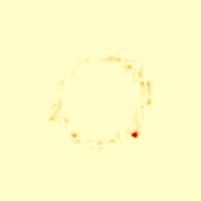
\includegraphics[width=0.33333333\figurewidth-1.3333333mm,
                             trim=30 30 30 100,
                             clip]
                            {images/data3/H_diff_down_36_rdoryl.png}
    };
    \node[bottom label] at (h_diff_down.south west) {
        $E^{\text{H}}_{\text{reconst}}$
    };
    \draw[dashed] (h_down.south west) -- (h_down.south east);



    \node[anchor=north, at={($(h_diff_lin.south) + (0, -1cm)$)}] (o2_orig) {
        
\includegraphics[width=0.33333333\figurewidth-1.3333333mm,
                         trim=105 25 15 95,
                         clip]
                        {images/O2_orig_rdoryl.png}
    };
    \node[top label] at (o2_orig.north west) {Original};

    \node[title] at (o2_orig.north west) {
        \textsc{\normalsize Syngas I: ${\text{O}_2}$}
    };

    \node[anchor=north, at={($(h_diff_knn.south) + (0, -1cm)$)}] (o2_1) {
        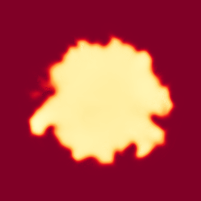
\includegraphics[width=0.33333333\figurewidth-1.3333333mm,
                         trim=105 25 15 95,
                         clip]
                        {images/O2_lin_1_rdoryl.png}
    };
    \node[top label] at (o2_1.north west) {$q=1,\,c=7.6$};

    \node[anchor=north, at={($(h_diff_down.south) + (0, -1cm)$)}] (o2_12) {
        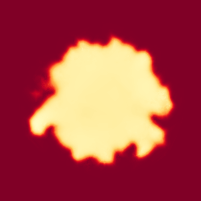
\includegraphics[width=0.33333333\figurewidth-1.3333333mm,
                         trim=105 25 15 95,
                         clip]
                        {images/O2_lin_12_rdoryl.png}
    };
    \node[top label] at (o2_12.north west) {$q=11.5,\,c=49$};

    \node[anchor=north, at={($(o2_orig.south) + (0, -2mm)$)}] (o2_23) {
        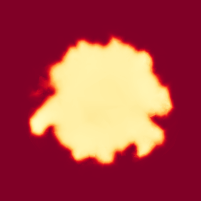
\includegraphics[width=0.33333333\figurewidth-1.3333333mm,
                         trim=105 25 15 95,
                         clip]
                        {images/O2_lin_23_rdoryl.png}
    };
    \node[top label] at (o2_23.north west) {$q=23.3,\,c=101$};

    \node[anchor=north, at={($(o2_1.south) + (0, -2mm)$)}] (o2_58) {
        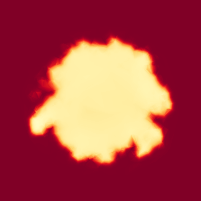
\includegraphics[width=0.33333333\figurewidth-1.3333333mm,
                         trim=105 25 15 95,
                         clip]
                        {images/O2_lin_58_rdoryl.png}
    };
    \node[top label] at (o2_58.north west) {$q=58,\,c=253$};

    \node[anchor=north, at={($(o2_12.south) + (0, -2mm)$)}] (o2_240) {
        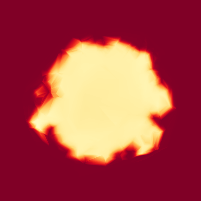
\includegraphics[width=0.33333333\figurewidth-1.3333333mm,
                         trim=105 25 15 95,
                         clip]
                        {images/O2_lin_240_rdoryl.png}
    };
    \node[top label] at (o2_240.north west) {$q=240,\,c=1037$};

\end{tikzpicture}
	\caption{
	Top: Comparison of reconstruction results for \ce{H} of \textsc{Syngas II}
 	with $q=\text{36}$ (ca. 2500 profile lines, $c=\text{321}$).
 	Bottom: Reconstruction results for \ce{O2} of \textsc{Syngas I} using linear
 	interpolation with different sample densities (detail view).}
	\label{fig:comp}
\end{figure}
%

We compared the results of linear and \ac{kANN} interpolation for reconstruction.
Our experiments show that for the \ac{kANN} interpolation a combination of five
nearest neighbors weighted with a Shepard weighting function using an exponent
of 20 gave the lowest errors. Therefore, we illustrate the results for these
parameters only.
%
% Since the \ac{kANN} interpolation uses Shepard weights, we have two parameters: $k$
% for the number of approximate nearest neighbors to consider, and $p$, which is
% the exponent in the Shepard weighting function. We computed the error for
% values of $k$ ranging from $5$ to $20$, and of $p$ ranging from $1$ to $20$. A
% combination of $k=5$ and $p=20$ yielded the best results. Therefore, we
% illustrate the results for these parameters.
%
We also compared our results to the error introduced by naively downsampling
the data to the same storage size needed by the sparse representation. This is
the currently established way of reducing the size of \ac{DNS} data. For
comparison with a dedicated compression algorithm, we used the well-established
\ac{3D}-\ac{SPIHT} algorithm~\cite{Kim2000} implemented in the QccPack
library~\cite{Fowler2000} on our data.

% To be able to evaluate the ability of the sparse form to accurately represent
% the original data, we must also compare it to the method used previously to
% reduce the size of DNS data: na\"{i}ve downsampling. For comparison, we
% downsampled the original data to the same storage size as our sparse
% representation, then upsampled it back to the original resolution. We then
% used the same metric $E^V_\text{reconst}$ to compute the error introduced by
% this process.

\Cref{fig:CRvMSE} shows the reduction ratio $c$ vs. the reconstruction
error $E_\text{reconst}^V$ for all tested methods for selected variables. Please
note that for \textsc{Syngas II}, higher reduction ratios are achieved than for
\textsc{Syngas I}, due to the flame in the former being relatively smaller. For
small reduction ratios, the downsampling approach naturally performs better,
because it does not introduce errors due to model assumptions. For higher
reduction ratios, which are needed in practice, our sparse representation always
performs significantly better. It is also apparent that linear interpolation
performs better than \ac{kANN} in almost all cases. As a dedicated compression
algorithm, \ac{3D}-\ac{SPIHT} achieves better reconstruction quality than our approach. It
is however necessary to decompress the data back to its full size before any
analysis can be carried out, thus losing a major advantage of our sparse
representation, which captures important data features by design.

\begin{figure}[t]
	\tikzset{external/export next=false}
	\setlength\figureheight{0.2\textheight}
	\setlength\figurewidth{0.8\textwidth}
	\centering
	% \hbox{\hspace{-1.5em}
	%
\pgfplotstableread[col sep=comma]{figures/compr_table.csv}\tabledata
\pgfplotstableread{figures/compr_table_900.csv}\tabledataII

% \definecolor{mycolor2}{rgb}{0, 0, 1}
% \definecolor{mycolor2}{rgb}{0.5, 0.5, 1}
% \definecolor{mycolor1}{rgb}{1, 0, 0}
% \definecolor{mycolor1}{rgb}{1, 0.5, 0.5}

\begin{tikzpicture}

\pgfplotsset{
	width=\figurewidth,
	height=\figureheight,
	scale only axis,
    every tick/.style={color=black, thin},
}

\begin{axis}[%
		font=\small,
		name = times
		axis y line* = left,
		axis x line* = box,
		tick pos = left,
		xmin=1,
		xmax=240,
		xmode=log,
		xminorticks=true,
		xlabel={$q$},
		every tick/.style={color=black, thin},
		ymin=1,
		ymax=500,
		ymode=log,
		ylabel={\textcolor{mycolor2}{$t[\text{min}]$}},
		% every axis y label/.style={ at={(rel axis cs:-0.07, 0.95)} },
		scaled y ticks = false,
		%legend style={legend pos = north west}
	]

	\addplot[
		color=mycolor2,
		dashed,
		thick
	]
	table[x = q, y expr = \thisrow{t_mean} + \thisrow{t_std}]{\tabledata};

	\addplot[
		color=mycolor2,
		dashed,
		thick
	]
	table[x = q, y expr = \thisrow{t_mean} - \thisrow{t_std}]{\tabledata};

	\addplot[
		color=mycolor2,
		solid,
		thick
	]
	table[x = q, y = t_mean]{\tabledata};

	\addplot[
		color=mycolor2,
		dashdotted,
		thick
	]
	table[x = q, y = t]{\tabledataII};

\end{axis}

\begin{axis}[% --- CF
		font=\small,
        xmin=1,
        xmax=240,
        xmode=log,
        ymin = 10,
        ymax = 1000,
        ymode=log,
        yminorticks=true,
        ticklabel pos=right,        
		axis y line* = right,
		axis x line = none,
		ylabel = {\textcolor{mycolor1}{$c$}},
		% every axis y label/.style={ at={(rel axis cs:1.05, 0.95)} },
		scaled y ticks = false,
    ]

    \addplot[
		color=mycolor1,
		dashed,
		thick
	]
	table[x = q, y expr = \thisrow{c_mean} + \thisrow{c_std}]{\tabledata};

	\addplot[
		color=mycolor1,
		dashed,
		thick
	]
	table[x = q, y expr = \thisrow{c_mean} - \thisrow{c_std}]{\tabledata};

	\addplot[
		color=mycolor1,
		solid,
		thick
	]
	table[x = q, y = c_mean]{\tabledata}; 

	\addplot[
		color=mycolor1,
		dashdotted,
		thick
	]
	table[x = q, y = c]{\tabledataII}; 
\end{axis}

\end{tikzpicture}
	% }
	\caption{
	Reduction ratio $c$ and computation time $t$ for different seeding densities
	q. Plot shows mean (solid) and standard deviation (dashed) over
	eight time steps of data set \textsc{Hydrogen} and values for the synthetic
	data set (dash-dotted).}
	\label{fig:compression_table}
	\Todo[inline]{Make synthetic line more distinct. Use inline tikz instead of
	text to describe pattern. Add minor ticks on right side.}
\end{figure}

To further illustrate the performance of our approach, we tested it on eight
time steps of the data set \textsc{Hydrogen}. This data set is from a turbulent
premixed spherical hydrogen flame and has a resolution of $\text{400}^3$ voxels
and 11 variables. This is a typical size for our cooperation partner. One time
step amounts to about 5 GB\Todo{Use SI units or similar to typeset memory sizes}
of data. The whole simulation has hundreds of thousands of time steps. Even
storing a fraction of them quickly results in terabytes of data. We selected
eight time steps from a late (most complex) stage of the simulation. Choosing
$q=\text{5}$, which retains very high accuracy for reconstruction,
we reduced them to about 30 MB each. This means only 0.6\% of the original
storage space is required.

For a scalability test, we generated a synthetic data set with $\text{900}^3$ voxels
and 11 variables. This is three times the maximum volume our cooperation
partner is able to simulate. We created noise based on an isotropic turbulence
frequency spectrum~\cite{Ferrante2003}. This noise was added to a low frequency
component to emulate larger flame structures with smaller surface pertubations.
Thresholding produces a surface on which average profiles of the different
variables were superimposed. Domain experts confirmed the similarity of the
result to real simulations, making it suitable for scalability tests.
Since each profile line has to be processed separately, the run time of the
algorithm is approximately linear in the number of seed points, and thus depends
indirectly on the flame surface area and structure.
\Cref{fig:compression_table} shows run times and compression ratios for
the synthetic data set and \textsc{Hydrogen}. Data set volume and flame surface
area of the synthetic data set are one order of magnitude higher than that of
\textsc{Hydrogen}. This results in a run time which is also one order of
magnitude higher, confirming the scalability of our approach.

We have shown that full scalar fields can be reconstructed with good agreement
to the original data from a sparse representation requiring a small fraction of
the storage space. This representation explicitly captures features such
as the points of steepest slope of reactants and products and the point
of maximum concentration of intermediate species. In the following section,
these feature points are used to visualize the relations between feature
surfaces of different variables.
%
% our compression approach maintains good quality while
% providing high reduction ratios. It also preserves features of the data such
% as the points of steepest slope of reactants and products as well as the point
% of maximum concentration of intermediate species. These feature points can now
% be used to visualize the relations between feature surfaces of different
% variables.
%
% subsection evaluation_compression (end)
%
% section reconstruction (end)
